\section{Zadanie 8}
Podłączając regulator bezpośrednio do obserwatora zamiast do obiektu otrzymujemy gorszą jakość regulacji, ale nie wymagającą mierzenia zmiennych stanu.
Wartość sygnału sterującego uległa znacznemu pogorszeniu.

\begin{figure}[H]
\centering
 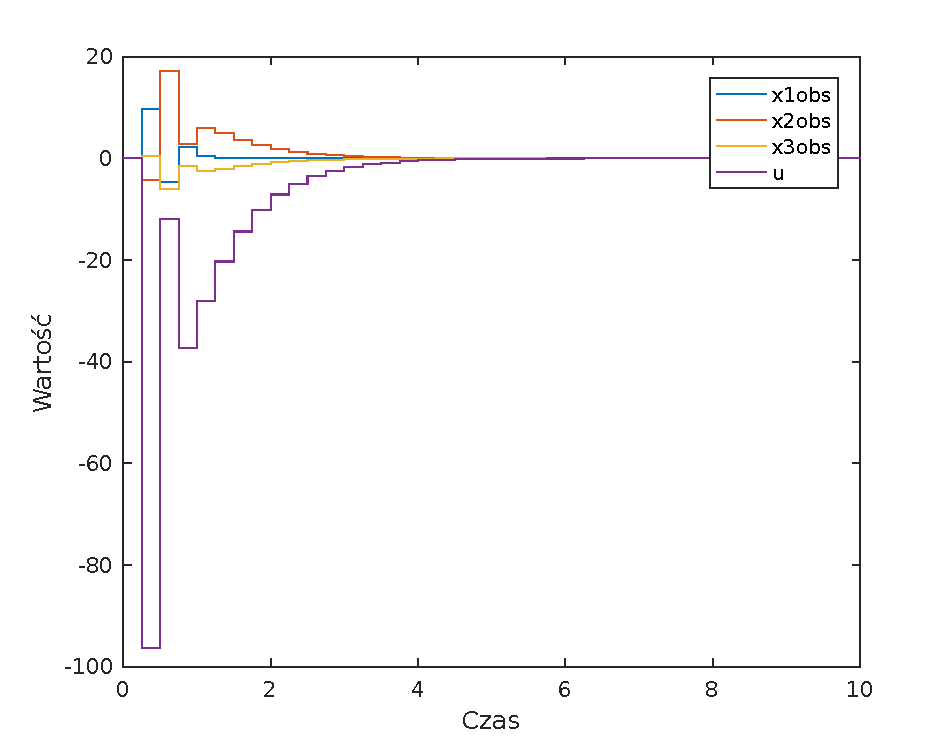
\includegraphics[width=\textwidth]{img/obsreg1.pdf}
\caption{Najszybszy obserwator $z_{o1}=z_{o2}=z_{o3}=0$ połączony z regulatorem $z_{b1}=0,3$, $z_{b2}=0,3$ i $z_{b3}=0,7$.}
\end{figure}

Można teraz spowolnić obserwator, aby przywrócić wartości $u(k)$ do akceptowalnych.

\begin{figure}[H]
\centering
 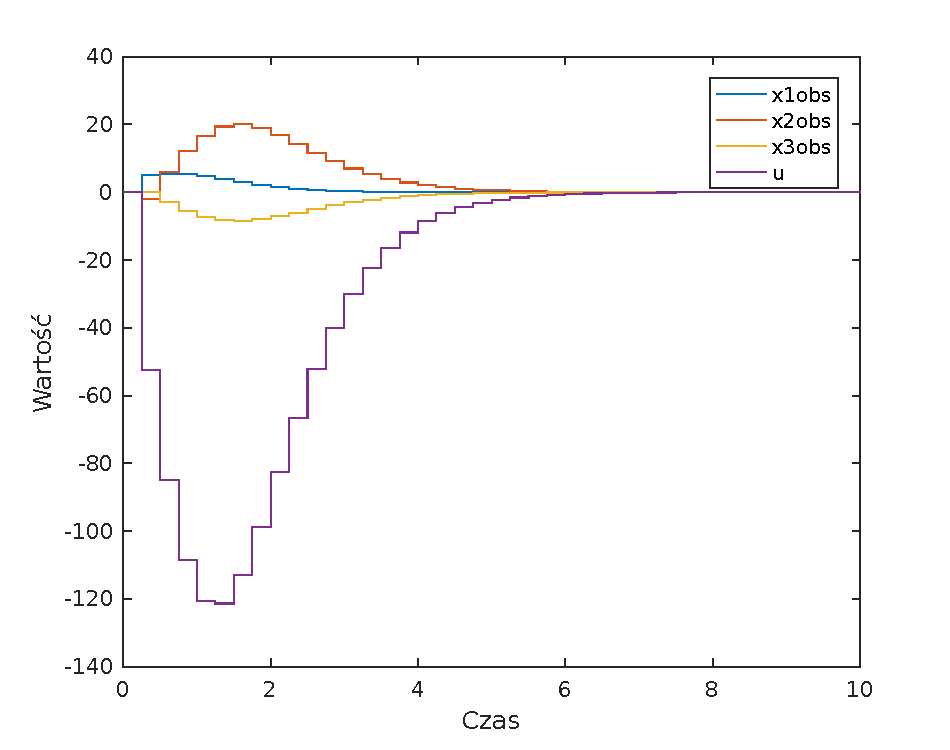
\includegraphics[width=\textwidth]{img/obsreg2.pdf}
\caption{Obserwator $z_{o1}=0,5$, $z_{o2}=0,5$ i $z_{o3}=0,5$.}
\end{figure}

Tak, jak poprzednim razem dążymy do tego, aby wartość sygnału sterującego nie oscylowała, jednocześnie zbiegając do zera wystarczająco szybko.
\begin{figure}[H]
\centering
 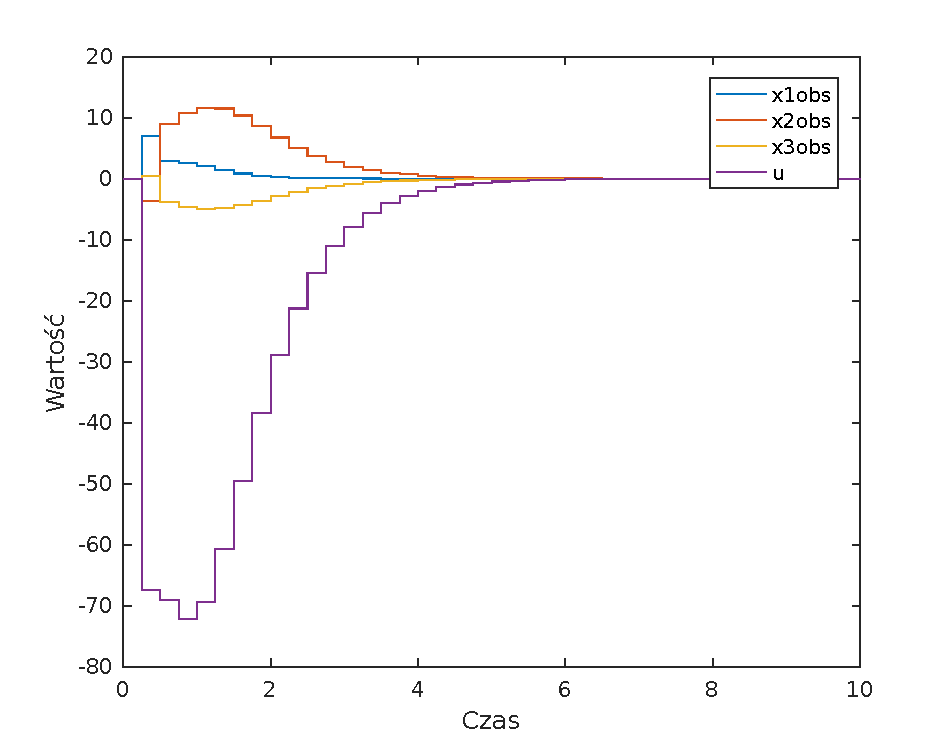
\includegraphics[width=\textwidth]{img/obsreg3.pdf}
\caption{Obserwator $z_{o1}=0,2$, $z_{o2}=0,2$ i $z_{o3}=0,5$.}
\end{figure}

Oprócz zmieniania biegunów obserwatora można także modyfikować i regulator.

\begin{figure}[H]
\centering
 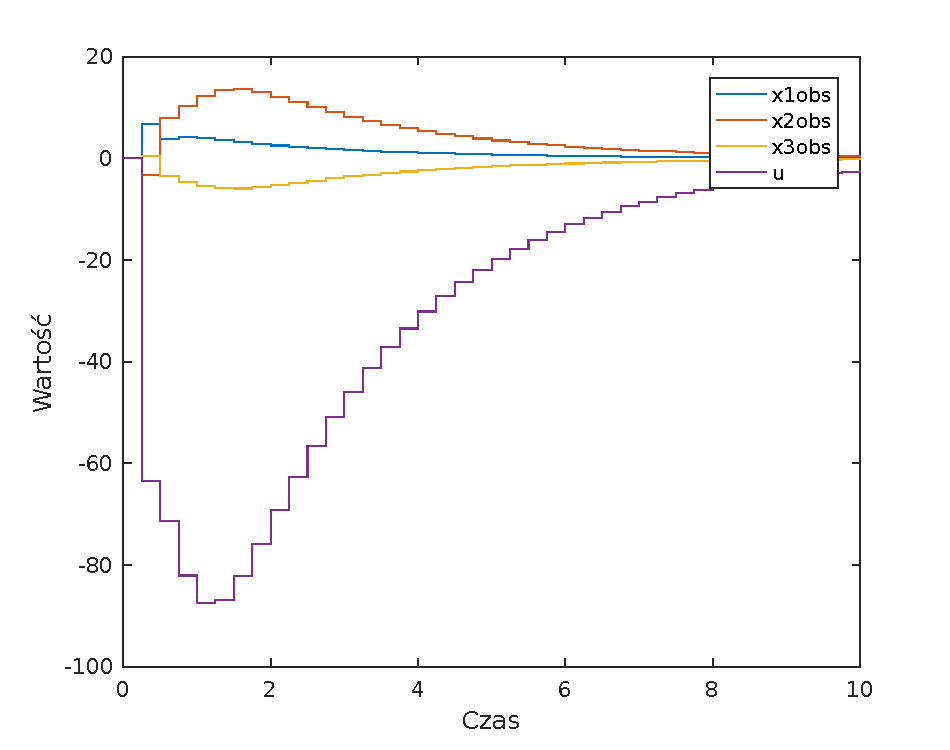
\includegraphics[width=\textwidth]{img/obsreg4.pdf}
\caption{Obserwator $z_{o1}=0,3$, $z_{o2}=0,3$ i $z_{o3}=0,4$, połączony z regulatorem $z_{b1}=0,2$, $z_{b2}=0,2$ i $z_{b3}=0,9$.}
\end{figure}

\begin{figure}[H]
\centering
 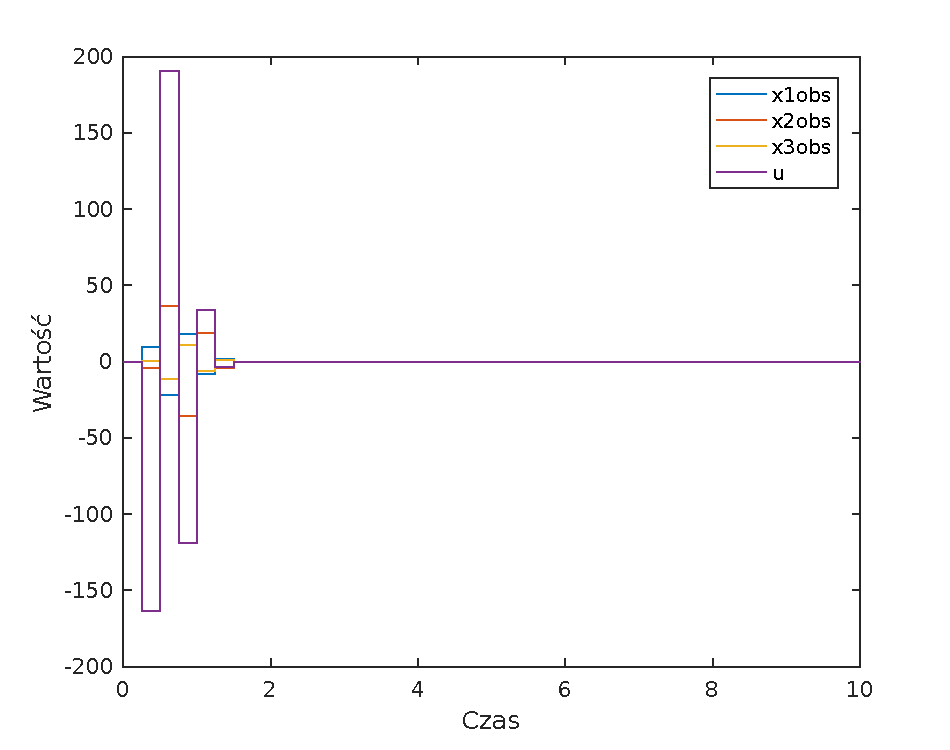
\includegraphics[width=\textwidth]{img/obsreg5.pdf}
\caption{Najszybszy układ --- obserwator $z_{o1}=z_{o2}=z_{o3}=0$ i regulator $z_{b1} = z_{b2} = z_{b3} = 0$.}
\end{figure}

\begin{figure}[H]
\centering
 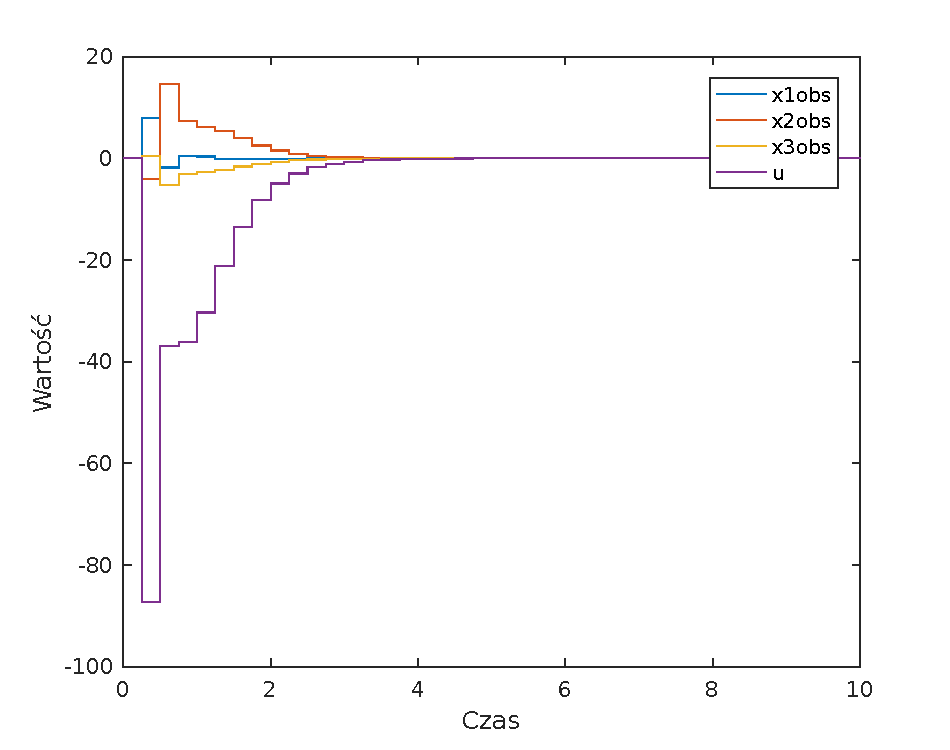
\includegraphics[width=\textwidth]{img/obsreg6.pdf}
\caption{Obserwator $z_{o1}=0,2$, $z_{o2}=0,2$ i $z_{o3}=0,6$, połączony z regulatorem $z_{b1}=0,2$, $z_{b2}=0,2$ i $z_{b3}=0,2$.}
\end{figure}

Zmiana regulatora wcale nie powoduje, że układ będzie lepiej pracował. 
Z eksperymentów wynika, że lepiej jest zostawić dobry regulator na takich ustawieniach, na jakich podłączony był oryginalnie do obiektu.
Następnie można modyfikować obserwator, aby $u(k)$ nie oscylowało i nie osiągało za wysokich wartości. Najlepsze znalezione ustawienia to:
\[
 \left\{
 \begin{array}{l}
 z_{b1}=0,3	\\
 z_{b2}=0,3	\\
 z_{b3}=0,7	\\
 z_{o1}=0,2	\\
 z_{o2}=0,2	\\
 z_{o3}=0,5	\\
 \end{array}
 \right.
\]
